\chapter{Walking through the demos}\index{Demos}
\label{ch:demos}

Let's go through some demos to clarify some of the concepts presented so far. The first demo consists of a set of simple artificial networks. Later, a more realistic scenario will be considered.

\section{Simple networks}

To build this set of networks, we first created a set of 20 nodes, regularly distributed through space.
 \begin{center}
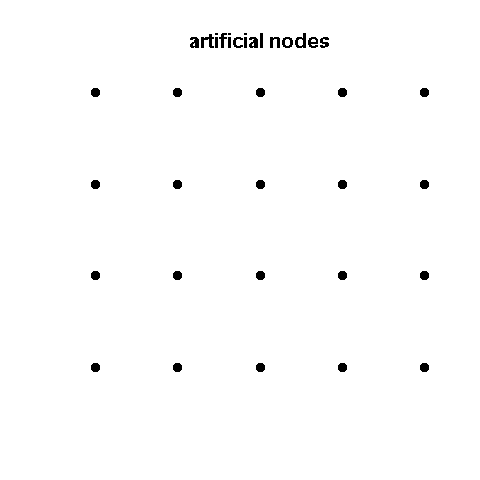
\includegraphics[scale=0.4]{nos.png}
%\caption{SIR-like models}
\label{fig:nos}
\end{center}

These nodes are called $N1$ to $N20$ and geocodes are equal to the numerical part of the node  name ($1$ to $20$). Each node is associated with a certain population. The .csv file containing this data is \textit{nodes20.csv}. The first few lines are:

\begin{verbatim}
"X","Y","Name","Pop","Geocode"
1,4,"N1",1000000,1
2,4,"N2",100000,2
3,4,"N3",1000,3
4,4,"N4",1000,4
5,4,"N5",1000,5
1,3,"N6",100000,6
2,3,"N7",1000,7
3,3,"N8",100000,8
4,3,"N9",100000,9
5,3,"N10",1000,10
1,2,"N11",1000,11
\end{verbatim}


Now, we create a set of 4 graphs, each graph connecting these 20 nodes in a different way. \textbf{Mesh} is a regular graph, with only local connections. \textbf{Star} represents a graph with two major hubs connected through a bridge. \textbf{Lin} could represent cities connected by a river, for example. \textbf{Tree} has a tree-like structure. The data for each set of edges are in the .csv files: mesh.csv, star.csv, lin.csv and tree.csv. 

\begin{center}
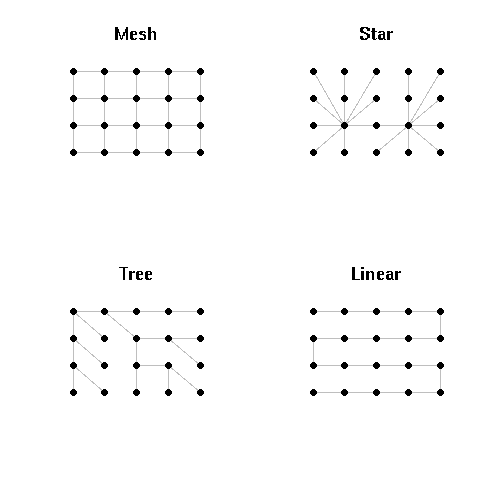
\includegraphics[scale=0.5]{artgraphs.png}
%\caption{SIR-like models}
\label{fig:artgraphs}
\end{center}

Now, a .epg script file must be prepared. The best way to do that is to edit an already existing .epg file. So, open \textbf{EpiGrass}, choose an .epg file and click on the \textbf{Edit} button. Your favorite editor will open and you can start editing. Don't forget to save it as a new file in your working directory. Of course, there is an infinite number of possibilities regarding the elaboration of the script. It all depends on the goals of the user. 

For the beginner, we suggest him/her to open the .epg files in this demo directory. They are all commented and may help the user in getting used with Epigrass language and capabilities.

\section{Using Epigrass for specific tasks}

\subsection{Describing a network}
A user wants to obtain the topological properties of a network. Reasons for this could be: 1) learn how to interpret these measures, 2) describe a air transportation or a road transportation network. To do that, you need:

\begin{description}
\item[Set steps = 1]. If no model of disease is needed, then most of the .epg script can be ignored. Don't remove anything, however, from the script.  Note that Epigrass requires a model in order to work properly, even if the user does not want it. One solution to reduce the run time, in this case, is to set \textbf{steps} to 1 (steps = number of steps in the simulation).
\item[Set MySQLout = 0]. Network measures are not sent to database.
\item[Set report = 1]. Report 1 calculates network measures and save them in a .pdf file.
\item[Especify siteRep]. If siteRep = [], only global network measures are included in the report. If site-specific measures are needed, include their geocodes in the list siteRep. For example, to calculate site stats for all nodes, mesh1.epg has:
\begin{verbatim}
report = 1
siteRep = [1,2,3,4,5,6,7,8,9,10,11,12,13,14,15,16,17,18,19,20]
\end{verbatim}
\end{description}

Script mesh1.epg is configured this way. Run it and take a look at the report. 


\subsection{Comparing networks}
A user wants to compare the properties of a set of networks. Reasons for this could be: 1) learn how to interpret these measures, 2) describe/compare a air transportation to a road transportation network, 3) analyse how network topology changes by adding/removing specific nodes or edges.

If there are four graphs, then four .epg files must be created. They all must set $report=1$ and $siteRep$ to the desired specification (as above). Each file must be executed and each one will provide a report. 

To quick thinks a little bit, the script allows the user to choose one of the files as a master file. In the option $BatchRun$, one may list the other scripts to be run after this one. They all must be in the same directory as the master file (or you may provide full path).

For example, suppose you want to compare the topologies of the four networks displayed in \ref{fig:artgraphs}. We created four files (mesh2.epg, star2.epg, lin2.epg, tree2.epg) and used one of them as master (mesh2.epg). The four files are exactly the same, except for the name of the edge file and the \textbf{Batch} specification. I.e., in mesh2.epg we specify:
\begin{verbatim}
Batch = ['star2.epg','lin2.epg','tree2.epg']
\end{verbatim}
Now, mesh2.epg is run. One report will be delivered for each script (In future version of Epigrass, a more integrated result is planned). From the reports, we get network measures for the four graphs (see table \ref{netstats}. These network measures are explained in chapter \ref{cap:analysis}). 

\begin{table}
\begin{center}
 \caption{Network measures for the demo networks: mesh, tree, star, lin}
\begin{tabular}{l r r r r}
\hline
Measure & mesh & tree & star & lin \\
\hline
number of nodes & 20 & 20 & 20 &\\
number of edges & 31 & 19  & 20 &  \\
cycles & 12 & 0 & 1 &\\
wiener distance & 1388 & 1540 & 860 &\\
mean distance & 3.65 & 4.05 & 2.26 &\\
diameter & 10 & 8 & 3 &\\
length & 280 & 136 & 258 &\\
weight & 124 & 66 & 63 &\\
Iota & 2.258 & 2.06 & 4.09 &\\
Pi & 4.827 & 2.428 & 6.45 &\\
Beta & 1.55 & 0.95 & 1 &\\
Alpha & 0.343 & 0 & 0.028 &\\
Gamma & 186 & 114 & 120 &\\
\hline
\end{tabular}
\label{netstats}
\end{center}
\end{table} 


\subsection{Simulate disease spread from a single site}
The user specifies a network (let's say, a tree network) and wishes to simulate disease spread in this network. The graph is disease-free at time 0. At time 1, an infected person arrives at site $N1$. No control measures are introduced. The model chosen is SipRpS. 
The script file tree3.epg was built following these guidelines:
\begin{description}
\item[Initial conditions] All individuals are initially susceptible, i.e.,  $S=N$.  
\item[Epidemic events] An infected individual arrives at time 1 in N1.
\item[steps=200] This may be increased or reduced, depending on the parameters.
\item[Report = 2]. Report 2 returns only the epidemiological results.
\item[Specify siteRep]. If site-specific measures are needed, include their geocodes in the list siteRep. For example, to calculate site stats for three nodes, tree3.epg has:
\begin{verbatim}
report = 2
siteRep = [1,12,14]
\end{verbatim}
Run this script and take a look at the report. A sugestion: change the script and seed the disease in a more central node. See how this affect the velocity of disease propagation.
\end{description}

 
\subsection{Simulating vaccination campaigns}
Vaccination may be simulated in different ways, using the section Epidemic Events in the script. These are some examples:
\begin{description}
\item[A single, local campaign].  In site N1, exactly at time 10, with coverage 0.5
\begin{verbatim}
Vaccinate = [(1,10,0.5)]
\end{verbatim}
\item[Simultaneous campaigns in three sites].  In sites N1, N4 and N6, exactly at time 10, with coverage 0.5
\begin{verbatim}
Vaccinate = [(1,10,0.5),(4,10,0.5),(6,10,0.5)]
\end{verbatim}
\item[Campaign with a time span].  In site N1, a campaign that occurs from day 10 to day 15, with daily coverage of 0.1.
\begin{verbatim}
Vaccinate = [(1,10,0.1),(1,11,0.1),(1,12,0.1),(1,13,0.1),
(1,14,0.1),(1,15,0.1)]
\end{verbatim}
\end{description}


\subsection{Simulating quarantines}
Quarantines are simulated similarly to vaccinations, but once they are initiated, they last until the end of the simulation (E ISSO?):
\begin{description}
\item[Quarantine in a single place].  In site N1, starting at time 10, with coverage 0.2
\begin{verbatim}
Quarantine = [(1,10,0.2)]
\end{verbatim}
\item[Quarantine in two places].  In sites N1 and N3, at times 10 and 12, respectively, with coverage 0.5
\begin{verbatim}
Quarantine = [(1,10,0.5),(3,12,0.5)]
\end{verbatim}
\item[Quarantine with a time span].  In site N1, a quarantine that starts at day 10 and ends at time 30, with daily coverage of 0.75.
\begin{verbatim}
Quarantine = [(1,10,0.75),(1,30,0)]
\end{verbatim}

\subsection{Comparing strategies}
One goal of modeling diseases is to compare alternative control measures in terms of number of cases prevented. A set of scripts were prepared to compare six alternative strategies for controlling the spread of an epidemic in the star graph, that was initiated at time 4 in site N1:
\begin{description}
\item[Strategy vac1]  Vaccinate site $N1$, at time $7$, with coverage $0.8$ .
\item[Strategy vac2]  Vaccinate sites $N1$, $N12$ and $N14$, at time $7$, with coverage $0.8$. $N12$ and $N14$ are central nodes of the star network and are natural candidates for vaccination.
\item[Strategy mixed] Strategy vac1 $+$ quarantine in sites $N12$ and $N14$, coverage of $0.7$.
\item[Strategy quar] Quarantine in sites $N1$, $N12$ and $N14$, coverage of $0.7$.
\end{description}
\begin{table}
\begin{center}
 \caption{Comparing control strategies for an epidemic in the star graph}
\begin{tabular}{l l l l}
\hline
Strategy & cases in $N1$ & cases in $N12$& total cases \\
\hline
None & & 3,345,668 & \\
vac1 & & & \\
vac2 & & & \\
mixed & & & \\
quar & & &\\
\hline
\end{tabular}
\label{strats}
\end{center}
\end{table} 


\end{description}




